%Notes by Harsh Mistry 
%CS 341
%Based on Template From  https://www.cs.cmu.edu/~ggordon/10725-F12/template.tex

\documentclass[twoside]{article}
\setlength{\oddsidemargin}{0.25 in}
\setlength{\evensidemargin}{-0.25 in}
\setlength{\topmargin}{-0.6 in}
\setlength{\textwidth}{6.5 in}
\setlength{\textheight}{8.5 in}
\setlength{\headsep}{0.75 in}
\setlength{\parindent}{0 in}
\setlength{\parskip}{0.1 in}
\usepackage{amsmath,amsfonts,graphicx}
\newcounter{lecnum}
\renewcommand{\thepage}{\thelecnum-\arabic{page}}
\renewcommand{\thesection}{\thelecnum.\arabic{section}}
\renewcommand{\theequation}{\thelecnum.\arabic{equation}}
\renewcommand{\thefigure}{\thelecnum.\arabic{figure}}
\renewcommand{\thetable}{\thelecnum.\arabic{table}}
\newcommand{\lecture}[4]{
   \pagestyle{myheadings}
   \thispagestyle{plain}
   \newpage
   \setcounter{lecnum}{#1}
   \setcounter{page}{1}
   \graphicspath{ {images/} }
   
   
%Info Box 
   \begin{center}
   \framebox{
      \vbox{\vspace{2mm}
    \hbox to 6.28in { {\bf CS 341 -  Algorithms
	\hfill Winter 2018} }
       \vspace{4mm}
       \hbox to 6.28in { {\Large \hfill Lecture #1: #2  \hfill} }
       \vspace{2mm}
       \hbox to 6.28in { {\it Lecturer: #3 \hfill Notes By: #4} }
      \vspace{2mm}}
   }
   \end{center}
   
   \markboth{Lecture #1: #2}{Lecture #1: #2}



 
}

\renewcommand{\cite}[1]{[#1]}
\def\beginrefs{\begin{list}%
        {[\arabic{equation}]}{\usecounter{equation}
         \setlength{\leftmargin}{2.0truecm}\setlength{\labelsep}{0.4truecm}%
         \setlength{\labelwidth}{1.6truecm}}}
\def\endrefs{\end{list}}
\def\bibentry#1{\item[\hbox{[#1]}]}

\newcommand{\fig}[3]{
			\vspace{#2}
			\begin{center}
			Figure \thelecnum.#1:~#3
			\end{center}
	}

\newtheorem{theorem}{Theorem}[lecnum]
\newtheorem{lemma}[theorem]{Lemma}
\newtheorem{ex}[theorem]{Example}
\newtheorem{proposition}[theorem]{Proposition}
\newtheorem{claim}[theorem]{Claim}
\newtheorem{corollary}[theorem]{Corollary}
\newtheorem{definition}[theorem]{Definition}
\newenvironment{proof}{{\bf Proof:}}{\hfill\rule{2mm}{2mm}}
\newcommand\E{\mathbb{E}}


%Start of Document 
\begin{document}

\lecture{5}{January 18, 2018}{Bin Ma}{Harsh Mistry}
 \section{Divide and Conquer Continued}
 \begin{ex} 2D Maxima \\
 Let \((x_i, y_i), i = 1, \ldots, n\) be \(n\) points on a two dimensional plane. A point \((x_i, y_i)\) dominates \((x_j, y_j)\) if \((x_i > x_j)\) and \(y_i > y_j\). A point \((x_i, y_i)\) is a 2D maximum if no other points dominate it. That is, for any \(j \neq i \), either \(x_j \leq x_i\), either \(x_j \leq x_i\) or \(y_j \leq y_i\)
 
\begin{center}
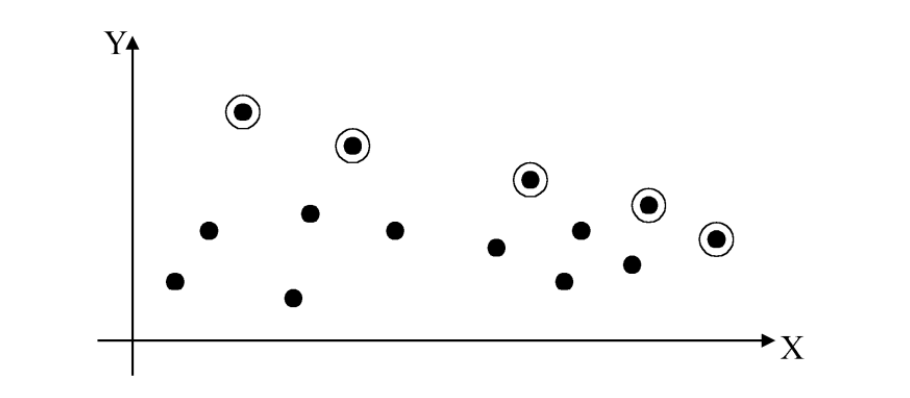
\includegraphics[scale=0.5]{2}\\
Taken from Bin Ma's Lecture Notes
\end{center}

if X and Y are treated as two different properties about a product. Then a maximum can provide some unique value proposition. However, a product that is dominated by some other products is hopeless. 

The problem is to find all maxima from n given points. We solve this by divide and conquer.

\begin{center}
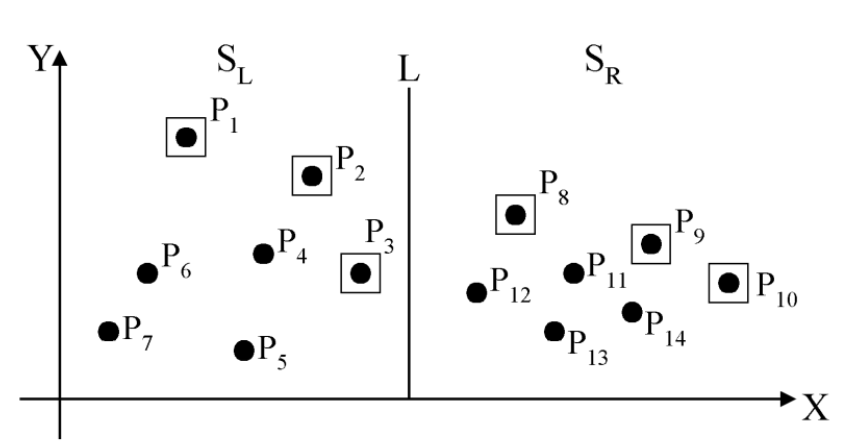
\includegraphics[scale=0.5]{3}\\
Taken from Bin Ma's Lecture Notes
\end{center}

For simplicity, lets assume points have different x-axis. (More general cases to be discussed later). Divide the points into two halves. 

Suppose the recursion returns the maxima from left and right halves, respectively. How do we construct the maxima of the whole point set?

First we notice that a maximum for the whole set must be a maximum of wither the left or the right halves. Secondly, the right maxima are already maxima of the whole set. Thirdly, a maximum of the left half is a maximum of the whole set if and only if its higher than all points at the right side. 

we this first sort all points to x-axis. This will take \(O(n \log n)\) time. Then the following algorithm will work. 

\textbf{Algorithm Maxima-DC}\\
Input : a list of points \((x_1, y_1), \ldots, (x_n, y_n)\) sorted across to x-axis

\begin{enumerate}
\item If \(n < 5\) solve the problem by definition and return the maxima 
\item Solve the first \(n/2\) and last \(n/2\) points recursively. Denote solutions be \(C_1\) and \(C_2\), respectively
\item Compute the largest y-axis in the last \(n/2\) points. Denote it \(m_y\)
\item Return \(C_2 \cup \{(x,y) \in C_1 \mid y \geq m_y\}\)
\end{enumerate}

The correctness follows from the above discussion. Detailed proof is left as an exercise  

Time complexity: \(T(n) = 2T(n/2) + n\) From Master theorem, \(T(n) = O(n \log n )\)

Now consider the slightly more general case where two points may have the same x-axis. We can reuse the same algorithm. The only difference is that when ordering two points with the same x-axis, we put the one with smaller y axis at left. 
One can verify that the same algorithm and same proof 
 
 
 
 \end{ex}

\end{document}





